\documentclass[12pt,a4paper]{article}
\usepackage{amsmath}	
\usepackage{graphicx}	

\begin{document}
\title{Kalman Filter Lecture Notes}
\author {Fadi Younes}
\maketitle
\newpage
\section*{Introduction}

The Kalman filter is a technique of mathematics, named after Rudolf E. Kalman. The aim is to use measurements observed over time, including noise (random variations) and other inconsistencies, and to generate values that appear to be equal to the true values of the measurements and their corresponding determined values. The Kalman method gives predictions of the true values of the observations and their associated measured values by estimating a value, measuring the variance of the expected value and computing a weighted average of the predicted value, and the value calculated\cite{zarchan2013fundamentals}.\\
\begin{figure}[h]
  \centering
 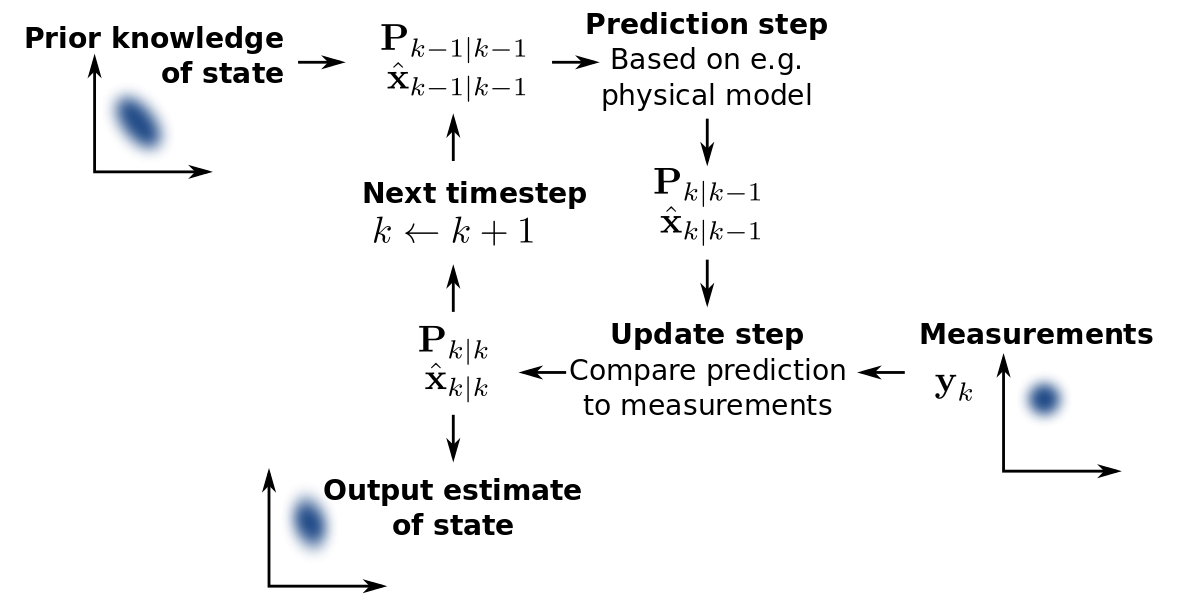
\includegraphics[width=3.4 in]{k.PNG}
  \caption{Basics of kalman Filtering}\label{1}
\end{figure}
\\As shown in Figure \ref{1}, the observed state ambiguity and expected value of observed state. The Updation of estimation is done by state transition measurements. $\hat{\mathbf{x}}_{k | k-1}$ is the system estimated state at 'k' time step and $\mathbf{P}_{k |k-1}$ represents uncertainty or ambiguity \cite{zarchan2013fundamentals}\cite{wolpert2000perception}.
\section*{Linear Quadratic Estimation}

The Kalman filter is most frequently called the linear quadratic estimation (LQE) in control systems. Kalman filter is used with linear quadratic regulator (LQR) to solve the control issues of linear quadratic gaussian controller (LQG). This filter and both the controllers are the basic solutions for most of the problems that occur in control systems \cite{klumb2006division}.\\
\section*{Dynamic System Model}

Kalman filters are based on time-domain-discrete linear dynamic systems. These are modelled on a Markov chain based on linear operators that are disturbed by Gaussian noise. There is a powerful duality seen between Kalman Filter equations and those of the Markov concealed model. To use the Kalman filter to approximate the internal performance of the process given just a pattern of noisy measurements, the process must be modelled according to the Kalman filter framework. \cite{li2019boundedness}\\
Kalman filter model suppose the true state at (k-1) as, k emerges from the origin.
\begin{equation}
\mathbf{x}_{k}=\mathbf{F}_{k} \mathbf{x}_{k-1}+\mathbf{B}_{k} \mathbf{u}_{k}+\mathbf{w}_{k}
\end{equation}
where,
\begin{itemize}
  \item $F_{k}$ is the Is the state transformation model applied to the preceding state x$_{k-1}$
  \item $B_{k}$ is the control-input configuration that is used for the uk control vector
  \item $W_{k}$ is the system noise that is presumed to be taken from the zero mean multivariate normal Qk covariance distribution.
\end{itemize}
This model does not exactly fit many real dynamic systems. The reason is that the influence of unmodelled dynamics relies on the input and can therefore lead to uncertainty with the estimation algorithm (it diverges).\\
\section*{Optimality and Efficiency}
The Kalman filter is the ideal linear filter when;
\begin{itemize}
  \item The framework fits in perfectly with the real system
  \item The noise that enters is pure (uncorrelated)
  \item Noise covariances are precisely identified
\end{itemize}
Once the covariances are approximated, evaluating the filter 's performance is effective; i.e., if the quality of the state estimation could be enhanced. The innovative technology sequence (the output prediction error) is a constant noise if the Kalman filter works efficiently, hence the whiteness property of the technology measures filter performance \cite{strid2009block}\\
\section*{Kalman Gain}
The Kalman filter is an estimator of minimal mean-square error. The error in the state estimation is given as \cite{ishihara2006robust}
\begin
{equation}\mathbf{x}_{k}-\hat{\mathbf{x}}_{k | k}
\end{equation}
The trace is minimized if the derivative vector with respect to the matrix of gain is zero. The gain found by this way is known as ideal or optimal gain which yields minimum mean square error (MMSE) estimates when used in any system.\\
\section{Non-Linear Filters}
The Kalman filter is restricted to a linear presumption. Nevertheless, more complex systems can be nonlinear. The nonlinearities could either be correlated with the research framework or the observation model, or even with both. There are two types of non-linear filters i.e. extended Kalman filter and unscented Kalman filter.
\subsection{Extended Kalman Filter}
The state transition and observation models must not be linear functions of the state in the extended Kalman filter (EKF), but may be (differentiable) functions instead.
\begin{equation}
\begin{array}{l}
\mathbf{x}_{k}=f\left(\mathbf{x}_{k-1}, \mathbf{u}_{k}\right)+\mathbf{w}_{k} \\
\mathbf{z}_{k}=h\left(\mathbf{x}_{k}\right)+\mathbf{v}_{k}
\end{array}
\end{equation}
The function f can be used to determine the future state from the previous calculation and likewise the function h can be used to determine the predicted measurement from the estimated condition. f and h cannot therefore be added directly to covariance. Instead it measures a matrix of partial derivatives (the Jacobian) \cite{maryak2004use}\\
The Jacobian is analyzed with current state predicted at every step size. Such matrix multiplication can be used in simulations of the Kalman filter. This process linearizes essentially the nonlinear function around the current prediction.\\
\subsection{Unscented Kalman Filter}
When the state transformation and observation framework i.e. the predicting and updating parameters f and h are extremely non-linear, the extended Kalman filter will produce especially poor performance. It is because the covariance is perpetuated by linearizing the associated nonlinear network.\\
The unscented Kalman filter (UKF) utilizes a stochastic testing technology called as the unscented transition to pick a minimal range of data points known as sigma points around the mean. Then, these sigma points are perpetuated through the nonlinear models, from which the estimated mean and covariance are then retrieved. The effect is a filter that captures the true mean and covariance with greater precision.\cite{terejanu2013discrete}\\
Additionally, this approach reduces the necessity for complex calculation of Jacobians, which can be a challenging task in itself for complex functions ( i.e. demanding difficult derivatives if accomplished analytically or if done statistically, becomes expensive way).\\
\bibliographystyle{ieeetran}
\bibliography{Ref_kalman}
\end{document}
